\documentclass{ximera}
\usepackage[colorlinks=true,urlcolor=blue]{hyperref}
\title{Setting up the repository}
\begin{document}
\begin{abstract}
Instructions for setting up a repository containing course materials.
\end{abstract}
\maketitle
\begin{enumerate}
\item Create a directory for your course files
and change to that directory.
In this example, we will create a directory called \verb!sampleCourse!.
\begin{center}
\begin{verbatim}
mkdir sampleCourse
cd sampleCourse 
\end{verbatim}
\end{center}
\item A Ximera course consists of a directory containing
a text file called \verb!course.xim!. This file should contain
the name of the course, a description of the course,
and the names of all the \LaTeX\ activity files in the order
they should be presented to students. In the example below
there is one activity file \verb!example.tex!
written without the extension \verb!.tex!
contained in a directory \verb!example!.
For more information about the structure of \verb!course.xim!
see the following activity.
\begin{verbatim}
---
name: Getting Started with Ximera
description: This is a Ximera activity explaining how to get started
with Ximera for instructors.
---

example/example
\end{verbatim}
In general, we recommend having each
activity in its own directory, which hasthe same name.
This facilitates the
sharing of activities between collaborators and makes reusing existing
activities much easier. Later in this course, we will see examples of
how to borrow existing activities from other courses
rather than starting from scratch.

\item As mentioned above, we need to add a directory
called \verb!example! containing a file called \verb!example.tex!.
\begin{verbatim}
mkdir example
cd example
touch example.tex
\end{verbatim}

\item The activity contained in \verb!example.tex!
should be in the document class \verb!ximera!
and should contain the title of the activity
and an abstract. For example,
\begin{verbatim}
\documentclass{ximera}
\title{The First Activity}
\begin{document}
\begin{abstract}
This activity deals with \verb!Ximera! activities
\end{abstract}
\maketitle
\end{document}
\end{verbatim}
The activity at this stage contains no content.

\item On \href{http://github.org}{\tt github.org}
create a repository as shown
in the image below.
\begin{image}
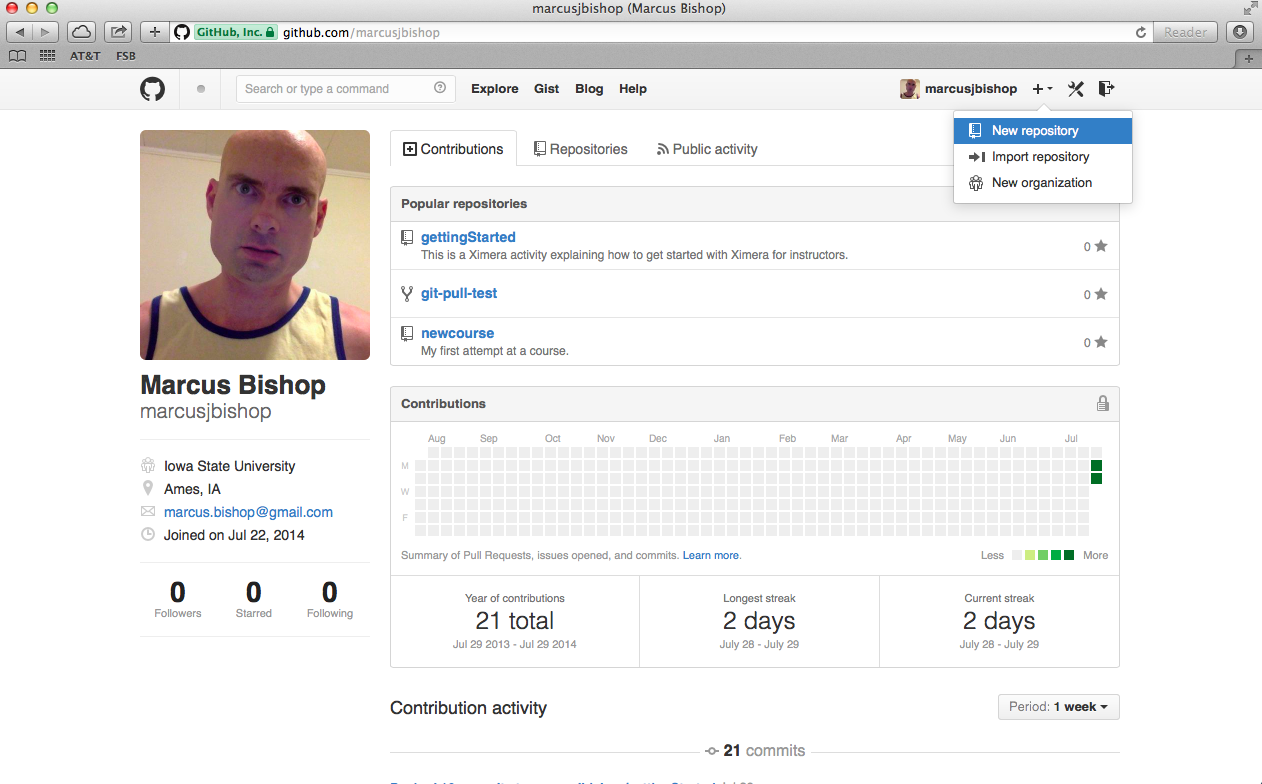
\includegraphics[scale=.3]{RepoInit.png}
\end{image}

\item Follow the instructions in \href{http://github.org}{\tt github.org} to set up
the repository, accepting all default settings.
This should involve executing some further \verb!git! commands that
connect and push your repository to
\href{http://github.org}{\tt github.org}:
\begin{verbatim}
touch README.md
git init
git add README.md
git commit -m "first commit"
git remote add origin https://github.com/marcusjbishop/example.git
git push -u origin master
\end{verbatim}
These commands also appear on \href{http://github.org}{\tt github.org}.

\item Write something in \verb!README.md!

\item Click on \verb!settings! on the
\href{http://github.org}{\tt github.org} page
for the repository created above,
and then on \verb!Webhooks & Services!
\begin{center}
\begin{image}
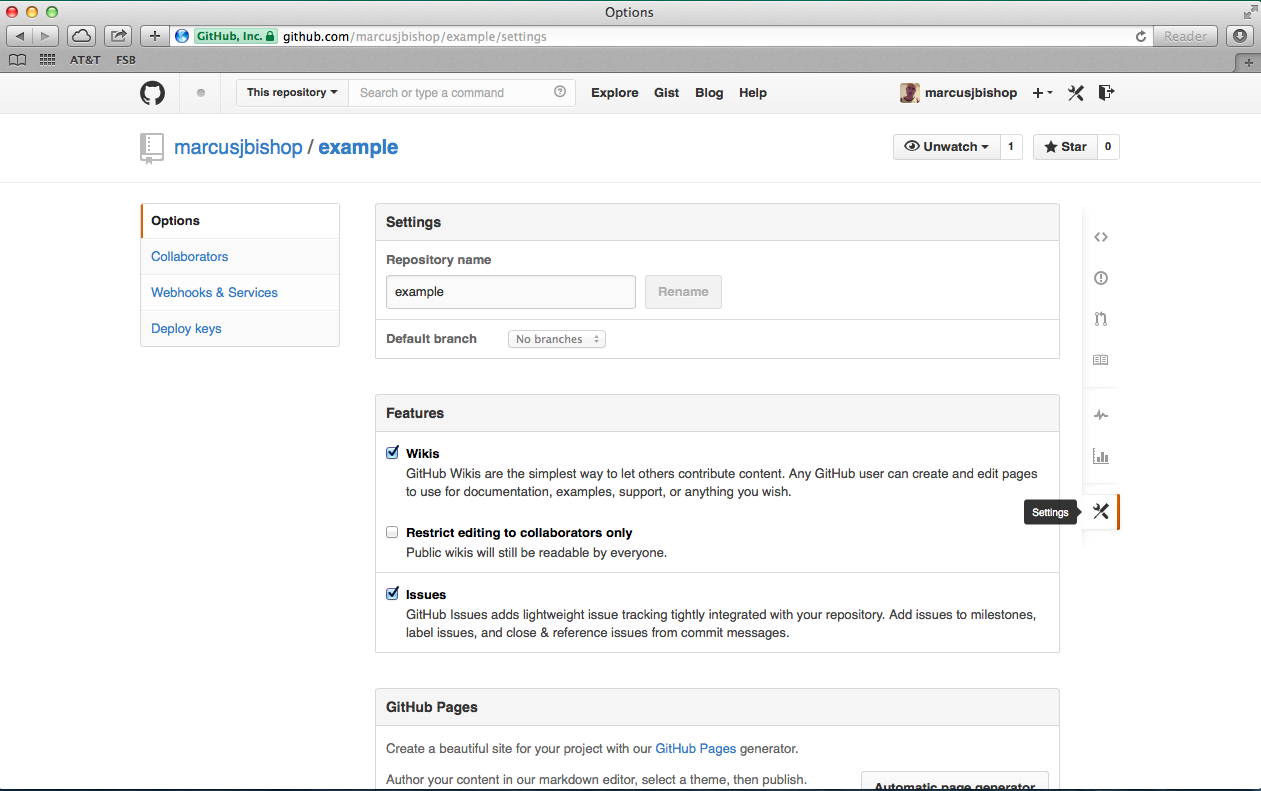
\includegraphics[scale=.3]{Webhook.png}
\end{image}
\end{center}
Now click the \verb!Add webhook! button.
Put \verb!http://ximera.osu.edu/github!
into the \verb!Payload URL! field and
\verb!8mi0tsrje9n3asPu86XC198G1XSdZj!
into the \verb!Secret! field.

\item In order to cause your course to appear on
\href{http://ximera.osu.edu/course}{\tt ximera.osu.edu/course}
you need to \verb!push! the repository.
However, since \verb!git! will not allow you to \verb!push!
until you make a change, this is a good point
to add an exercise to \verb!exercise.tex!. For example,
you could edit the file as shown below.
\begin{verbatim}
\documentclass{ximera}
\title{The First Activity}
\begin{document}
\begin{abstract}
This activity deals with \verb!Ximeara! activities.
\end{abstract}
\maketitle
This activity is about creative work.
\begin{exercise}
  Choose the best place to work on mathematics.
  \begin{multiple-choice}
    \choice{At the library}
    \choice[correct]{At the caf\'e}
    \choice{In your office}
  \end{multiple-choice}
\end{exercise}
\end{document}
\end{verbatim}
See the following activity for more information on creating
exercises.

\item Change to the root directory of your repository
and execute the following commands.
\begin{verbatim}
git commit -am "Added an exercise"
git push
\end{verbatim}

\item If everything went well, you should find your course listed at 
\href{http://ximera.osu.edu/course}{\tt ximera.osu.edu/course}.
If not, see the troubleshooting activity.
\end{enumerate}
\end{document}
